\chapter{Chapter 5 --- Phase 2: Downstream Impact Under Honest
Evaluation}\label{chapter-5-phase-2-downstream-impact-under-honest-evaluation}

Chapter 4 established that SZZ labels are noisy, that the noise is
class-conditional, and that variants share failure modes. None of that
tells us whether the noise \emph{matters}. A model might be robust to
it; a metric might be insensitive to it; the effect might be smaller
than the variance between projects.

This chapter answers \textbf{RQ2}: how does the choice of SZZ label
source shift measured JIT-SDP performance across evaluation regimes of
increasing realism?

Its central finding is not the one the research question anticipates.
The label source matters, but \textbf{the evaluation protocol matters
more}, and the largest single effect in the entire study is an artefact
of how the field scores its models rather than of which labels it trains
them on.

\section{5.1 Method}\label{method}

\subsection{5.1.1 The design}\label{the-design}

Phase 2 is a four-way factorial grid.

\begin{longtable}[]{@{}
  >{\raggedright\arraybackslash}p{(\linewidth - 2\tabcolsep) * \real{0.5000}}
  >{\raggedright\arraybackslash}p{(\linewidth - 2\tabcolsep) * \real{0.5000}}@{}}
\toprule\noalign{}
\begin{minipage}[b]{\linewidth}\raggedright
Dimension
\end{minipage} & \begin{minipage}[b]{\linewidth}\raggedright
Levels
\end{minipage} \\
\midrule\noalign{}
\endhead
\bottomrule\noalign{}
\endlastfoot
\textbf{Model} & LApredict, JITLine, ORB \\
\textbf{Training label source} & Reference labels + six SZZ variants
(7) \\
\textbf{Evaluation regime} & Naive \emph{k}-fold, chronological,
chronological-online, prequential-with-latency (4) \\
\textbf{Scoring convention} & Oracle-scored, self-scored (2) \\
\end{longtable}

Twenty-one projects, ten random seeds, giving \textbf{16,380 evaluation
records}.

\textbf{Models.} LApredict is logistic regression on a single feature
--- lines added --- included because prior work has found such baselines
competitive with deep models, making it a test of whether measured
effects are properties of the task or of model capacity. JITLine is a
100-tree random forest with SMOTE oversampling and threshold moving,
representing the high-capacity batch state of the practice. ORB is a
20-member online logistic ensemble with Poisson oversampling whose rate
responds to the model's recent prediction bias; it is the only model of
the three that can operate on a stream.

\textbf{Regimes}, in increasing order of realism:

\begin{enumerate}
\def\labelenumi{\arabic{enumi}.}
\tightlist
\item
  \textbf{Naive \emph{k}-fold} --- random 10-fold cross-validation,
  ignoring commit order. Included precisely because it is indefensible:
  a model may train on 2020 commits and be tested on 2015 ones. It is
  the regime most widely used in the JIT-SDP literature, which is why it
  is the baseline rather than the strawman.
\item
  \textbf{Chronological} --- a single 50/50 split in commit-timestamp
  order. Removes temporal leakage; retains the assumption that all
  training labels are available at training time.
\item
  \textbf{Chronological-online} --- ORB trained sequentially on the
  first half, then frozen and evaluated on the second. Isolates the
  learner change from the regime change.
\item
  \textbf{Prequential with verification latency} --- test-then-train
  streaming. Each commit is predicted when it arrives, and its label is
  delivered only when it would actually have become known.
\end{enumerate}

\subsection{5.1.2 The scoring convention, and why it is the
experiment}\label{the-scoring-convention-and-why-it-is-the-experiment}

The distinction between \emph{oracle-scored} and \emph{self-scored} is
the conceptual core of this chapter.

\begin{itemize}
\tightlist
\item
  \textbf{Self-scored} --- the model is evaluated against the same noisy
  SZZ labels it was trained on. \textbf{This is what the JIT-SDP
  literature does.}
\item
  \textbf{Oracle-scored} --- the model is trained on SZZ labels but
  evaluated against the independently constructed reference labels, held
  out and never used in training.
\end{itemize}

Self-scoring measures how faithfully a model reproduces a heuristic.
Oracle-scoring measures how well it identifies what the reference calls
defect-introducing. These are different quantities, and the field
reports the first while interpreting it as the second. Holding out an
independently sourced scoring key makes the gap between them measurable,
and measuring that gap is the purpose of Phase 2.

\subsection{5.1.3 Verification latency}\label{verification-latency}

Under the prequential regime, a defect label is not available when the
commit arrives; it becomes available when the defect is found and fixed.
The timeline implemented is:

\begin{itemize}
\tightlist
\item
  At commit time \emph{t}: the model predicts; the prediction is scored
  immediately against the reference label.
\item
  If the training label is clean: delivered as a training example at
  \emph{t + W}, with \emph{W} = 90 days.
\item
  If defective and the fix arrives within the window: delivered as a
  positive at the fix time.
\item
  If defective but the fix arrives later: delivered \textbf{first as a
  negative at \emph{t + W}, then corrected to positive at the fix time.}
\item
  If defective with no linked fix: delivered as a negative at \emph{t +
  W} and never corrected.
\end{itemize}

The third case is what makes latency more than a delay. A model
operating under a 90-day window does not merely wait for labels ---
\textbf{it is actively trained on labels it will later learn were
wrong.} On this corpus, 53.0\% of defect labels arrive after the window,
with a median latency of 113 days.

\subsection{5.1.4 Statistical protocol}\label{statistical-protocol}

Every test is paired at the \textbf{project} level, \emph{n} = 21, with
seeds averaged before pairing. Pooling over the 16,380 records would be
pseudo-replication: the seeds are not independent observations of
anything.

Each comparison reports a Wilcoxon signed-rank \emph{p}-value, a
\textbf{matched-pairs rank-biserial correlation} (the proportion of
projects moving in the effect's direction, derived from the same signed
ranks as the \emph{p}-value), a \textbf{Hodges--Lehmann} location
estimate, and a percentile bootstrap confidence interval computed for
the Hodges--Lehmann statistic itself.

Seventy-four tests were run. Multiplicity is corrected twice:
\textbf{within test family}, and \textbf{globally across all 74}. The
global column exists because the families were defined during analysis
rather than declared in advance, so a sceptic could argue the grouping
was chosen to favour the results. A claim surviving global Holm needs no
defence of how families were drawn. Thirty-two tests survive
within-family correction; \textbf{twenty-one survive global correction},
and it is the global column that the headline claims rest on.

\textbf{Both phases reported here are exploratory and are labelled as
such throughout.} No hypothesis in this report was pre-registered, which
is why the global multiplicity correction is reported alongside the
within-family one.

\section{5.2 Results}\label{results}

\subsection{5.2.1 The full matrix}\label{the-full-matrix}

Mean MCC over 21 projects \ensuremath{\times} 10 seeds.

\textbf{Batch models}

\begin{longtable}[]{@{}
  >{\raggedright\arraybackslash}p{(\linewidth - 10\tabcolsep) * \real{0.1667}}
  >{\raggedright\arraybackslash}p{(\linewidth - 10\tabcolsep) * \real{0.1667}}
  >{\raggedright\arraybackslash}p{(\linewidth - 10\tabcolsep) * \real{0.1667}}
  >{\raggedright\arraybackslash}p{(\linewidth - 10\tabcolsep) * \real{0.1667}}
  >{\raggedright\arraybackslash}p{(\linewidth - 10\tabcolsep) * \real{0.1667}}
  >{\raggedright\arraybackslash}p{(\linewidth - 10\tabcolsep) * \real{0.1667}}@{}}
\toprule\noalign{}
\begin{minipage}[b]{\linewidth}\raggedright
Model
\end{minipage} & \begin{minipage}[b]{\linewidth}\raggedright
Labels
\end{minipage} & \begin{minipage}[b]{\linewidth}\raggedright
\emph{k}-fold oracle-scored
\end{minipage} & \begin{minipage}[b]{\linewidth}\raggedright
\emph{k}-fold \textbf{self}-scored
\end{minipage} & \begin{minipage}[b]{\linewidth}\raggedright
Chrono oracle-scored
\end{minipage} & \begin{minipage}[b]{\linewidth}\raggedright
Chrono \textbf{self}-scored
\end{minipage} \\
\midrule\noalign{}
\endhead
\bottomrule\noalign{}
\endlastfoot
\textbf{JITLine} & \textbf{reference} & \textbf{0.2430} & --- &
\textbf{0.1016} & --- \\
JITLine & B-SZZ & 0.1751 & \textbf{0.4129} & \textbf{0.1324} & 0.2232 \\
JITLine & AG-SZZ & 0.1164 & 0.3037 & 0.0904 & 0.1351 \\
JITLine & MA-SZZ & 0.1272 & 0.3295 & 0.0786 & 0.1395 \\
JITLine & L-SZZ & 0.1391 & 0.2434 & 0.0804 & 0.1482 \\
JITLine & R-SZZ & 0.1131 & 0.1801 & 0.0626 & 0.0920 \\
JITLine & RA-SZZ & 0.1164 & 0.3070 & 0.0857 & 0.1402 \\
\textbf{LApredict} & \textbf{reference} & \textbf{0.2058} & --- &
\textbf{0.1734} & --- \\
LApredict & B-SZZ & 0.1941 & 0.3510 & 0.1634 & 0.2918 \\
LApredict & AG-SZZ & 0.2003 & 0.2472 & 0.1685 & 0.1975 \\
LApredict & MA-SZZ & 0.1995 & 0.2626 & 0.1664 & 0.2003 \\
LApredict & L-SZZ & 0.2078 & 0.2679 & 0.1706 & 0.2174 \\
LApredict & R-SZZ & 0.2016 & 0.1779 & 0.1731 & 0.1666 \\
LApredict & RA-SZZ & 0.2000 & 0.2603 & 0.1679 & 0.2143 \\
\end{longtable}

\emph{Reference-trained cells have no separate self-scored value: the
two conventions coincide by construction.}

\textbf{Online model (ORB)}

\begin{longtable}[]{@{}
  >{\raggedright\arraybackslash}p{(\linewidth - 8\tabcolsep) * \real{0.2000}}
  >{\raggedright\arraybackslash}p{(\linewidth - 8\tabcolsep) * \real{0.2000}}
  >{\raggedright\arraybackslash}p{(\linewidth - 8\tabcolsep) * \real{0.2000}}
  >{\raggedright\arraybackslash}p{(\linewidth - 8\tabcolsep) * \real{0.2000}}
  >{\raggedright\arraybackslash}p{(\linewidth - 8\tabcolsep) * \real{0.2000}}@{}}
\toprule\noalign{}
\begin{minipage}[b]{\linewidth}\raggedright
Labels
\end{minipage} & \begin{minipage}[b]{\linewidth}\raggedright
Chrono-online oracle
\end{minipage} & \begin{minipage}[b]{\linewidth}\raggedright
Chrono-online self
\end{minipage} & \begin{minipage}[b]{\linewidth}\raggedright
Prequential (time-avg)
\end{minipage} & \begin{minipage}[b]{\linewidth}\raggedright
Prequential (terminal)
\end{minipage} \\
\midrule\noalign{}
\endhead
\bottomrule\noalign{}
\endlastfoot
\textbf{reference} & \textbf{0.0777} & --- & \textbf{0.0970} & 0.0685 \\
B-SZZ & 0.0767 & 0.1613 & 0.0578 & 0.0566 \\
L-SZZ & 0.0082 & 0.0695 & 0.0582 & 0.0209 \\
RA-SZZ & 0.0193 & 0.0673 & 0.0395 & 0.0184 \\
AG-SZZ & 0.0177 & 0.0684 & 0.0365 & 0.0125 \\
MA-SZZ & 0.0216 & 0.0717 & 0.0353 & \textbf{\ensuremath{-}0.0030} \\
R-SZZ & 0.0114 & 0.0349 & 0.0315 & 0.0104 \\
\end{longtable}

Two features of this table are worth marking before the analysis.

First, \textbf{LApredict --- logistic regression on one feature --- is
the best model in the corpus under a chronological split} (0.1734
against JITLine's 0.1016 on reference labels). The random forest's
advantage exists only under \emph{k}-fold.

Second, MA-SZZ's apparently harmful negative MCC (\ensuremath{-}0.0030) exists only
under the terminal estimator; under the time-averaged estimator it is
+0.0353. \textbf{No MCC is quoted anywhere in this report without naming
the estimator}, and \S{}5.2.5 explains why.

\subsection{5.2.2 The inflation ladder}\label{the-inflation-ladder}

\begin{longtable}[]{@{}
  >{\raggedright\arraybackslash}p{(\linewidth - 6\tabcolsep) * \real{0.2500}}
  >{\raggedright\arraybackslash}p{(\linewidth - 6\tabcolsep) * \real{0.2500}}
  >{\raggedright\arraybackslash}p{(\linewidth - 6\tabcolsep) * \real{0.2500}}
  >{\raggedright\arraybackslash}p{(\linewidth - 6\tabcolsep) * \real{0.2500}}@{}}
\toprule\noalign{}
\begin{minipage}[b]{\linewidth}\raggedright
Step
\end{minipage} & \begin{minipage}[b]{\linewidth}\raggedright
Configuration
\end{minipage} & \begin{minipage}[b]{\linewidth}\raggedright
MCC
\end{minipage} & \begin{minipage}[b]{\linewidth}\raggedright
What was removed
\end{minipage} \\
\midrule\noalign{}
\endhead
\bottomrule\noalign{}
\endlastfoot
0 & JITLine, B-SZZ labels, \emph{k}-fold, self-scored & \textbf{0.4129}
& --- (the literature's configuration) \\
1 & JITLine, B-SZZ labels, \emph{k}-fold, oracle-scored & 0.1751 &
Circular self-scoring (\textbf{\ensuremath{-}0.238}) \\
2 & JITLine, reference labels, chronological & 0.1016 & Temporal
leakage \\
3 & ORB, reference labels, prequential + latency & \textbf{0.0970} &
Batch-to-stream \\
\end{longtable}

\textbf{A number that reads as 0.41 under the field's standard protocol
is 0.10 under a defensible one.}

\begin{figure}
\centering
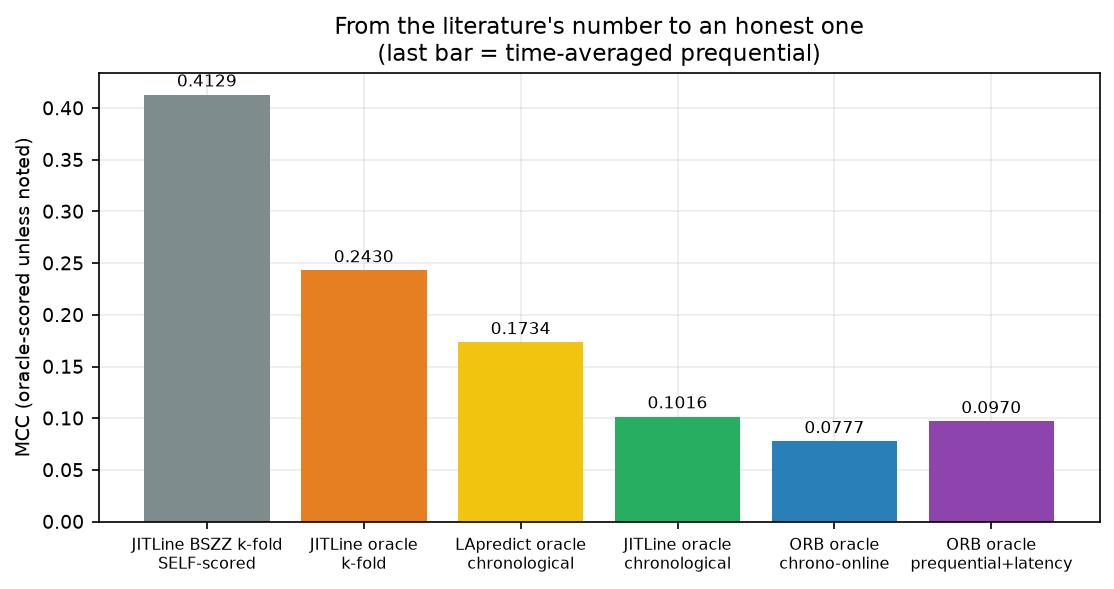
\includegraphics[width=\linewidth,keepaspectratio]{figures/f2_inflation_ladder.png}
\label{fig:f2_inflation_ladder}
\caption{The inflation ladder --- from the literature's configuration to
a defensible one}
\end{figure}

\textbf{Figure 5.1 --- Reading the figure.} Each bar is the same
prediction task measured under progressively more honest conditions,
left to right. The grey bar is what the field's protocol reports; the
rightmost bar is what survives realistic evaluation. \textbf{The height
difference between the first and last bar is this report in one
picture.}

The ladder must be read as \textbf{descriptive, not causal}. Step 3
changes the learner, the regime and the evaluation window
simultaneously, so the steps cannot be attributed to any one of them.
\S{}5.3 takes that apart.

\subsection{5.2.3 Result 1 --- Temporal leakage inflates, in proportion
to model
capacity}\label{result-1-temporal-leakage-inflates-in-proportion-to-model-capacity}

Random \emph{k}-fold against a chronological split, paired by project.
Fourteen comparisons: seven label sources \ensuremath{\times} two batch models.

\begin{longtable}[]{@{}
  >{\raggedright\arraybackslash}p{(\linewidth - 16\tabcolsep) * \real{0.1111}}
  >{\raggedright\arraybackslash}p{(\linewidth - 16\tabcolsep) * \real{0.1111}}
  >{\raggedright\arraybackslash}p{(\linewidth - 16\tabcolsep) * \real{0.1111}}
  >{\raggedright\arraybackslash}p{(\linewidth - 16\tabcolsep) * \real{0.1111}}
  >{\raggedright\arraybackslash}p{(\linewidth - 16\tabcolsep) * \real{0.1111}}
  >{\raggedright\arraybackslash}p{(\linewidth - 16\tabcolsep) * \real{0.1111}}
  >{\raggedright\arraybackslash}p{(\linewidth - 16\tabcolsep) * \real{0.1111}}
  >{\raggedright\arraybackslash}p{(\linewidth - 16\tabcolsep) * \real{0.1111}}
  >{\raggedright\arraybackslash}p{(\linewidth - 16\tabcolsep) * \real{0.1111}}@{}}
\toprule\noalign{}
\begin{minipage}[b]{\linewidth}\raggedright
Model
\end{minipage} & \begin{minipage}[b]{\linewidth}\raggedright
Labels
\end{minipage} & \begin{minipage}[b]{\linewidth}\raggedright
\emph{k}-fold
\end{minipage} & \begin{minipage}[b]{\linewidth}\raggedright
Chrono
\end{minipage} & \begin{minipage}[b]{\linewidth}\raggedright
HL
\end{minipage} & \begin{minipage}[b]{\linewidth}\raggedright
95\% CI
\end{minipage} & \begin{minipage}[b]{\linewidth}\raggedright
Rank-biserial
\end{minipage} & \begin{minipage}[b]{\linewidth}\raggedright
Holm (family)
\end{minipage} & \begin{minipage}[b]{\linewidth}\raggedright
Holm (global)
\end{minipage} \\
\midrule\noalign{}
\endhead
\bottomrule\noalign{}
\endlastfoot
\textbf{JITLine} & \textbf{reference} & 0.2430 & 0.1016 &
\textbf{+0.1373} & {[}+0.1046, +0.1721{]} & \textbf{+1.000} &
\textbf{1.3e-05} & \textbf{7.1e-05} \\
JITLine & L-SZZ & 0.1391 & 0.0804 & +0.0667 & {[}+0.0216, +0.0900{]} &
+0.792 & \textbf{0.0094} & \textbf{0.0389} \\
JITLine & R-SZZ & 0.1131 & 0.0626 & +0.0515 & {[}+0.0258, +0.0764{]} &
+0.706 & 0.0393 & 0.1607 \\
LApredict & reference & 0.2058 & 0.1734 & +0.0339 & {[}+0.0006,
+0.0647{]} & +0.489 & 0.4015 & 1.000 \\
\end{longtable}

\emph{(Four of fourteen shown; the remainder follow the same pattern.)}

The headline is JITLine on reference labels: \textbf{+0.1373 MCC, with a
rank-biserial of exactly +1.000 --- all 21 projects, without exception.}
The exact test saturates.

\textbf{The effect scales with model capacity.} JITLine loses 0.137;
LApredict loses 0.034 and does not survive correction. A single-feature
logistic regression has little capacity to exploit temporal leakage; a
100-tree forest has a great deal.

\begin{quote}
This is the most damaging form the finding could take. The inflation is
largest exactly where the field reports its strongest results, so
\textbf{the apparent superiority of high-capacity models over simple
baselines is partly an artefact of the evaluation protocol that measures
it.}
\end{quote}

\subsection{5.2.4 Result 2 --- Self-scoring inflates further, and it is
model-dependent}\label{result-2-self-scoring-inflates-further-and-it-is-model-dependent}

Thirty-six comparisons: for each (model, label source, regime), the same
predictions scored against the training labels versus against the
reference.

\begin{longtable}[]{@{}
  >{\raggedright\arraybackslash}p{(\linewidth - 16\tabcolsep) * \real{0.1111}}
  >{\raggedright\arraybackslash}p{(\linewidth - 16\tabcolsep) * \real{0.1111}}
  >{\raggedright\arraybackslash}p{(\linewidth - 16\tabcolsep) * \real{0.1111}}
  >{\raggedright\arraybackslash}p{(\linewidth - 16\tabcolsep) * \real{0.1111}}
  >{\raggedright\arraybackslash}p{(\linewidth - 16\tabcolsep) * \real{0.1111}}
  >{\raggedright\arraybackslash}p{(\linewidth - 16\tabcolsep) * \real{0.1111}}
  >{\raggedright\arraybackslash}p{(\linewidth - 16\tabcolsep) * \real{0.1111}}
  >{\raggedright\arraybackslash}p{(\linewidth - 16\tabcolsep) * \real{0.1111}}
  >{\raggedright\arraybackslash}p{(\linewidth - 16\tabcolsep) * \real{0.1111}}@{}}
\toprule\noalign{}
\begin{minipage}[b]{\linewidth}\raggedright
Model
\end{minipage} & \begin{minipage}[b]{\linewidth}\raggedright
Labels
\end{minipage} & \begin{minipage}[b]{\linewidth}\raggedright
Regime
\end{minipage} & \begin{minipage}[b]{\linewidth}\raggedright
Self
\end{minipage} & \begin{minipage}[b]{\linewidth}\raggedright
Oracle
\end{minipage} & \begin{minipage}[b]{\linewidth}\raggedright
HL
\end{minipage} & \begin{minipage}[b]{\linewidth}\raggedright
95\% CI
\end{minipage} & \begin{minipage}[b]{\linewidth}\raggedright
Rank-biserial
\end{minipage} & \begin{minipage}[b]{\linewidth}\raggedright
Holm (global)
\end{minipage} \\
\midrule\noalign{}
\endhead
\bottomrule\noalign{}
\endlastfoot
\textbf{JITLine} & \textbf{B-SZZ} & \emph{k}-fold & 0.4129 & 0.1751 &
\textbf{+0.2303} & {[}+0.1886, +0.2784{]} & \textbf{+0.991} &
\textbf{1.0e-04} \\
JITLine & MA-SZZ & \emph{k}-fold & 0.3295 & 0.1272 & +0.1985 &
{[}+0.1393, +0.2648{]} & \textbf{+1.000} & \textbf{1.0e-04} \\
JITLine & RA-SZZ & \emph{k}-fold & 0.3070 & 0.1164 & +0.1861 &
{[}+0.1221, +0.2523{]} & \textbf{+1.000} & \textbf{1.0e-04} \\
JITLine & AG-SZZ & \emph{k}-fold & 0.3037 & 0.1164 & +0.1797 &
{[}+0.1201, +0.2456{]} & \textbf{+1.000} & \textbf{1.0e-04} \\
LApredict & B-SZZ & \emph{k}-fold & 0.3510 & 0.1941 & +0.1549 &
{[}+0.1213, +0.2029{]} & +0.957 & \textbf{6.0e-04} \\
LApredict & AG-SZZ & \emph{k}-fold & 0.2472 & 0.2003 & +0.0510 &
{[}\ensuremath{-}0.0123, +0.1100{]} & +0.351 & 1.000 \\
LApredict & R-SZZ & \emph{k}-fold & 0.1779 & 0.2016 & \textbf{\ensuremath{-}0.0238} &
{[}\ensuremath{-}0.0662, +0.0265{]} & \ensuremath{-}0.221 & 1.000 \\
\end{longtable}

\textbf{+0.2303 MCC is the largest effect in this report.} It is also
the effect with the clearest methodological reading: a random forest
trained on B-SZZ labels appears roughly two and a half times better at
finding defects than it is, because it is being graded by the heuristic
that taught it.

\begin{figure}
\centering
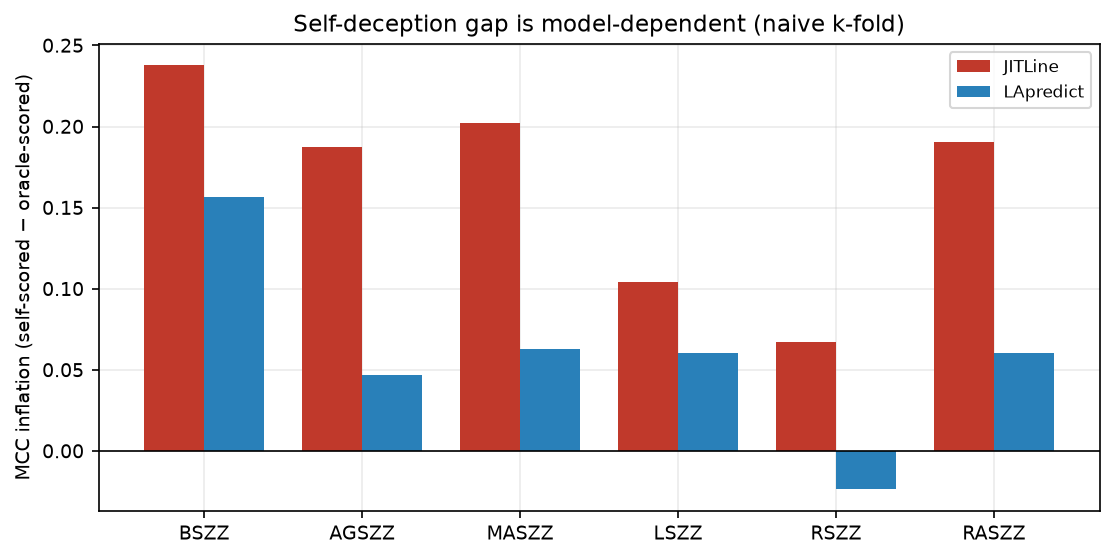
\includegraphics[width=\linewidth,keepaspectratio]{figures/f3_self_deception.png}
\label{fig:f3_self_deception}
\caption{Self-scoring gap by variant and model}
\end{figure}

\textbf{Figure 5.2 --- Reading the figure.} Each bar is how far a
model's apparent score \emph{drops} when it stops being graded against
the heuristic that trained it and is graded against the reference
instead. Red is JITLine (high capacity), blue LApredict (low capacity).
\textbf{The red bars are consistently much taller} --- the gap is a
capacity phenomenon.

\textbf{The gap is model-dependent, and the pattern is diagnostic.}
Under JITLine it is large and significant for every one of the six
variants. Under LApredict it is significant only for B-SZZ, and for
R-SZZ it is \emph{negative}. A single-feature logistic regression cannot
memorise a heuristic's idiosyncrasies; a high-capacity forest can.
\textbf{The self-scoring gap is a capacity phenomenon, which is exactly
what one would predict if the mechanism is a model fitting the error
structure of its labels.}

\textbf{The mechanism, tested directly.} That reading was, until
recently, an interpretation the gap was \emph{consistent with} rather
than one it established. We therefore tested it: restricting to the
8,060 B-SZZ-flagged commits and asking whether a model can separate
B-SZZ's false positives from its true positives using the same 14
features.

\begin{longtable}[]{@{}ll@{}}
\toprule\noalign{}
& Mean AUC \\
\midrule\noalign{}
\endhead
\bottomrule\noalign{}
\endlastfoot
Random forest, chronological split per project & \textbf{0.599} \\
Same pipeline, training labels permuted (the null) & 0.514 \\
\end{longtable}

Paired across projects: \textbf{HL +0.088, CI {[}+0.041, +0.131{]},
17/21 projects, \emph{p} = 0.0016.}

SZZ's errors carry structure the features can detect, so a model
\emph{can} fit them. The mechanism is real. \textbf{It is also weak ---
an AUC of 0.60 is modest separability --- and the +0.230 gap is almost
certainly not explained by this structure alone.} The claim this report
makes is ``the error structure is learnable'', not ``SZZ's mistakes are
easy to predict''.

\subsection{5.2.5 Result 3 --- Under realistic streaming, the label
source
matters}\label{result-3-under-realistic-streaming-the-label-source-matters}

Under the prequential regime with real verification latency, ORB trained
on reference labels against ORB trained on each variant, all scored
against the reference.

\begin{longtable}[]{@{}
  >{\raggedright\arraybackslash}p{(\linewidth - 14\tabcolsep) * \real{0.1250}}
  >{\raggedright\arraybackslash}p{(\linewidth - 14\tabcolsep) * \real{0.1250}}
  >{\raggedright\arraybackslash}p{(\linewidth - 14\tabcolsep) * \real{0.1250}}
  >{\raggedright\arraybackslash}p{(\linewidth - 14\tabcolsep) * \real{0.1250}}
  >{\raggedright\arraybackslash}p{(\linewidth - 14\tabcolsep) * \real{0.1250}}
  >{\raggedright\arraybackslash}p{(\linewidth - 14\tabcolsep) * \real{0.1250}}
  >{\raggedright\arraybackslash}p{(\linewidth - 14\tabcolsep) * \real{0.1250}}
  >{\raggedright\arraybackslash}p{(\linewidth - 14\tabcolsep) * \real{0.1250}}@{}}
\toprule\noalign{}
\begin{minipage}[b]{\linewidth}\raggedright
Reference vs
\end{minipage} & \begin{minipage}[b]{\linewidth}\raggedright
Mean gap
\end{minipage} & \begin{minipage}[b]{\linewidth}\raggedright
HL
\end{minipage} & \begin{minipage}[b]{\linewidth}\raggedright
95\% CI
\end{minipage} & \begin{minipage}[b]{\linewidth}\raggedright
Rank-biserial
\end{minipage} & \begin{minipage}[b]{\linewidth}\raggedright
Projects
\end{minipage} & \begin{minipage}[b]{\linewidth}\raggedright
Holm (family)
\end{minipage} & \begin{minipage}[b]{\linewidth}\raggedright
Holm (global)
\end{minipage} \\
\midrule\noalign{}
\endhead
\bottomrule\noalign{}
\endlastfoot
R-SZZ & +0.0655 & +0.0603 & {[}+0.0418, +0.0816{]} & +0.948 & 19/21 &
\textbf{0.0001} & \textbf{0.0009} \\
MA-SZZ & +0.0617 & +0.0638 & {[}+0.0390, +0.0845{]} & +0.896 & 18/21 &
\textbf{0.0003} & \textbf{0.0042} \\
AG-SZZ & +0.0605 & +0.0600 & {[}+0.0290, +0.0851{]} & +0.818 & 17/21 &
\textbf{0.0009} & \textbf{0.0243} \\
RA-SZZ & +0.0575 & +0.0577 & {[}+0.0357, +0.0808{]} & +0.879 & 18/21 &
\textbf{0.0004} & \textbf{0.0064} \\
\textbf{B-SZZ} & +0.0392 & \textbf{+0.0412} & {[}+0.0219, +0.0521{]} &
+0.879 & 18/21 & \textbf{0.0004} & \textbf{0.0064} \\
L-SZZ & +0.0388 & +0.0341 & {[}+0.0140, +0.0552{]} & +0.723 & 16/21 &
\textbf{0.0025} & 0.1241 \\
\end{longtable}

All six intervals exclude zero; \textbf{five of six survive global Holm
correction.}

\begin{figure}
\centering
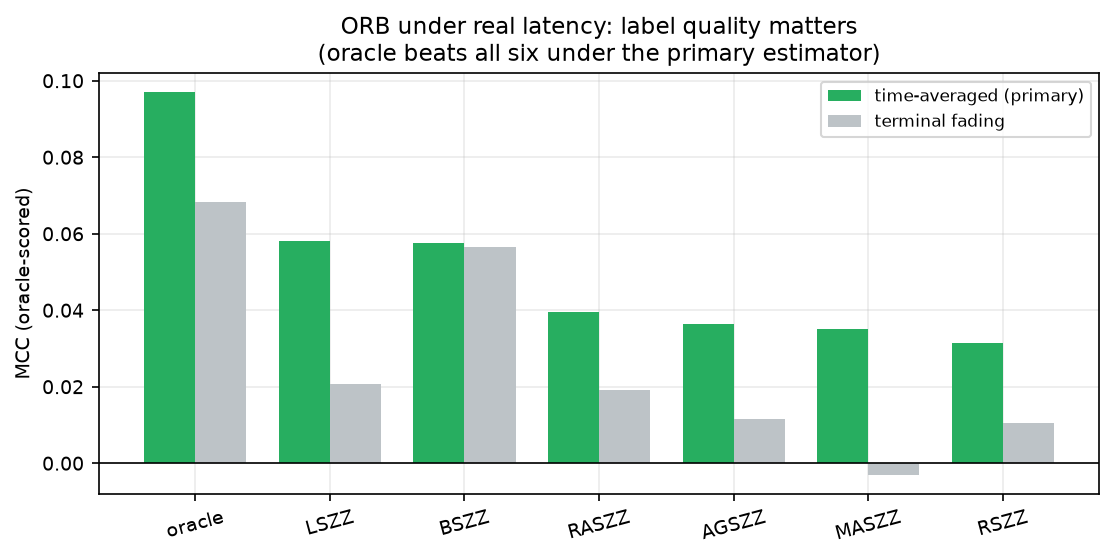
\includegraphics[width=\linewidth,keepaspectratio]{figures/f4_label_source.png}
\label{fig:f4_label_source}
\caption{Label source comparison under both prequential estimators}
\end{figure}

\textbf{Figure 5.3 --- Reading the figure.} Green bars are the primary
time-averaged estimator; grey the secondary terminal estimator. The
reference labels are leftmost and tallest under both. Note that MA-SZZ
dips below zero under the grey bars only --- an artefact of the noisier
statistic, not a model that actively harms.

\textbf{The B-SZZ comparison is the most informative row.} Because the
reference and B-SZZ share the same blame step and differ only in which
lines seed it (\S{}4.1.1), this contrast is a near-controlled ablation of
tangled commits. Its value is \textbf{+0.041 MCC, CI {[}+0.022,
+0.052{]}} --- a defensible estimate of what knowing which lines in a
fix actually fix the bug is worth to a deployed online learner.

\textbf{The gap does not track recall.} The correlation between a
variant's oracle-versus-variant gap and its recall is \ensuremath{-}0.18. L-SZZ
(recall 0.267) and B-SZZ (recall 0.641) have almost identical gaps.
Whatever drives the penalty, it is not simply how many defects the
labeller finds. This report cannot say what does drive it: \S{}6.2 names
the experiment that would.

\textbf{Estimator dependence, reported rather than buried.} Two
summaries of the prequential MCC trajectory are available: a
\emph{terminal} value computed from a fading confusion matrix (effective
window \ensuremath{\approx} 100 commits), and the \emph{time-averaged} mean of the
trajectory. They agree on every comparison in this report except one:
under the terminal estimator the B-SZZ row alone loses significance. The
time-averaged estimator is treated as primary on a measured basis ---
roughly half the project-level variance (0.051 against 0.092) --- and
\textbf{not} by appeal to a standard. MCC is not a decomposable loss, so
the prequential-with-fading construction does not extend to it directly;
both summaries are ad-hoc, and this report says so rather than claiming
canonical status for either.

\begin{figure}
\centering
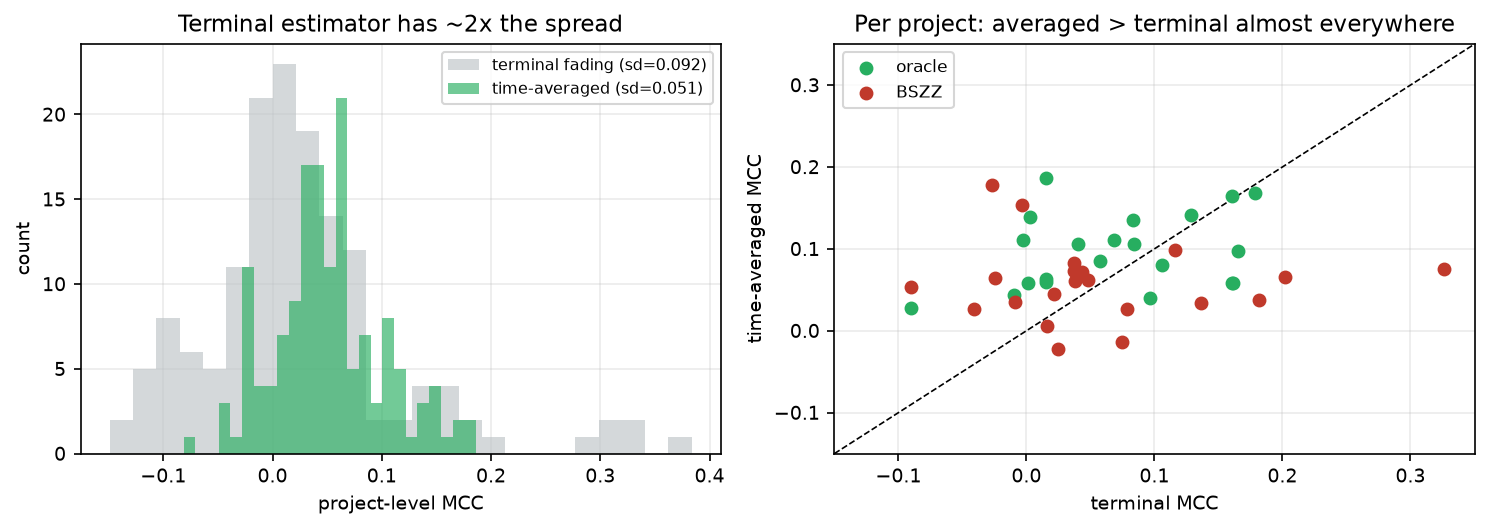
\includegraphics[width=\linewidth,keepaspectratio]{figures/f7_estimators.png}
\label{fig:f7_estimators}
\caption{Why the two estimators differ --- variance and per-project
comparison}
\end{figure}

\textbf{Figure 5.4 --- Reading the figure.} \emph{Left:} the spread of
project-level scores under each estimator --- the terminal distribution
is visibly wider, which is the measured basis for preferring the
time-averaged value. \emph{Right:} each project plotted under both;
points above the diagonal are projects where the time-averaged value is
higher.

\section{5.3 Sizing the latency effect: an unidentified contrast, and
the design that replaced
it}\label{sizing-the-latency-effect-an-unidentified-contrast-and-the-design-that-replaced-it}

The inflation ladder invites an obvious follow-up question. Step 3 costs
very little --- 0.1016 to 0.0970 --- so how much of the drop from batch
to streaming performance is attributable to verification latency
specifically?

\textbf{Read directly off the ladder, the answer would be about 9\%.
That reading is not valid, and the reason is worth setting out}, because
the same trap is available to anyone comparing a batch result against a
streaming one.

The contrast is \textbf{not identified}. Moving between those two rows
changes three things at once: the learner (forest \ensuremath{\rightarrow} online ensemble),
the label timing (immediate \ensuremath{\rightarrow} delayed), and the evaluation window (a
held-out second half \ensuremath{\rightarrow} the whole stream). Any one of the three could
produce the observed difference, and no arithmetic on those two numbers
can separate them.

A 2\ensuremath{\times}2 factorial that \textbf{does} isolate them --- learner (frozen /
adaptive) crossed with labels (immediate / delayed) --- gives:

\begin{longtable}[]{@{}lll@{}}
\toprule\noalign{}
Contrast & Estimate & Interval \\
\midrule\noalign{}
\endhead
\bottomrule\noalign{}
\endlastfoot
Latency effect & \ensuremath{\approx} +0.023 & contains zero \\
Adaptivity effect & \ensuremath{\approx} \ensuremath{-}0.046 & contains zero \\
Interaction & --- & contains zero \\
\end{longtable}

\textbf{Every contrast, including the interaction, has a confidence
interval spanning zero.} With 21 paired projects, effects below roughly
0.04 MCC are not resolvable, and these fall in that range.

\begin{figure}
\centering
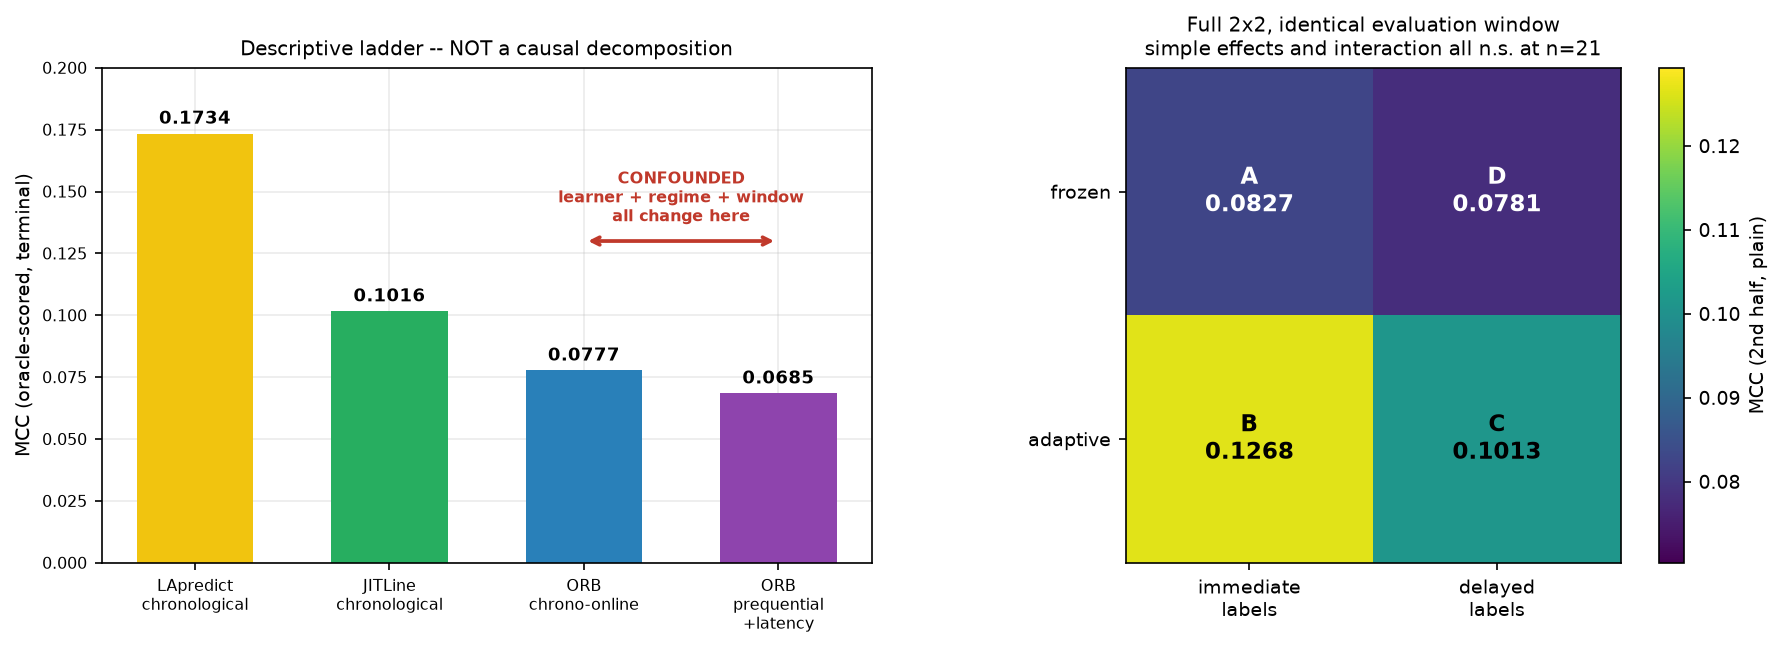
\includegraphics[width=\linewidth,keepaspectratio]{figures/f5_decomposition.png}
\label{fig:f5_decomposition}
\caption{The confounded ladder step, and the 2\ensuremath{\times}2 built to separate it}
\end{figure}

\textbf{Figure 5.5 --- Reading the figure.} \emph{Left:} the descriptive
ladder with the problematic step marked --- learner, regime and
evaluation window all change there at once. \emph{Right:} the 2\ensuremath{\times}2 that
separates them, brighter meaning higher MCC. The cells are close enough
that no contrast resolves.

So the conclusion is that \textbf{21 paired projects cannot resolve this
decomposition}, and it is reported as unresolved rather than as a null
--- the effect may well be real and simply smaller than this design can
detect.

\textbf{What this establishes for the work that follows.} A factorial on
the label source is the wrong instrument: it buys identification at the
cost of power, because every cell is a different learner on a different
stream. The alternative is to \textbf{hold the learner fixed by
construction} and vary only the noise, injecting controlled label errors
into a single source rather than switching between sources. That design
also needs a true no-latency control --- an arm in which \emph{every}
label, positive and negative, arrives immediately --- because a
fixed-delay arm is not one: it delays the 91.5\% majority class as
heavily as the minority, so comparing two delayed arms tests sensitivity
to the arrival \emph{schedule} rather than to delay itself. \S{}6.2.3
carries this forward.

\section{5.3b An exploratory finding: the JITLine
anomaly}\label{b-an-exploratory-finding-the-jitline-anomaly}

One result in the Phase 2 matrix runs against the chapter's argument and
is reported because it does.

Under chronological evaluation, \textbf{B-SZZ-trained JITLine (0.1324)
beats reference-trained JITLine (0.1016)}, winning in \textbf{15 of 21
projects}. Training on demonstrably noisier labels produces a better
model.

\begin{figure}
\centering
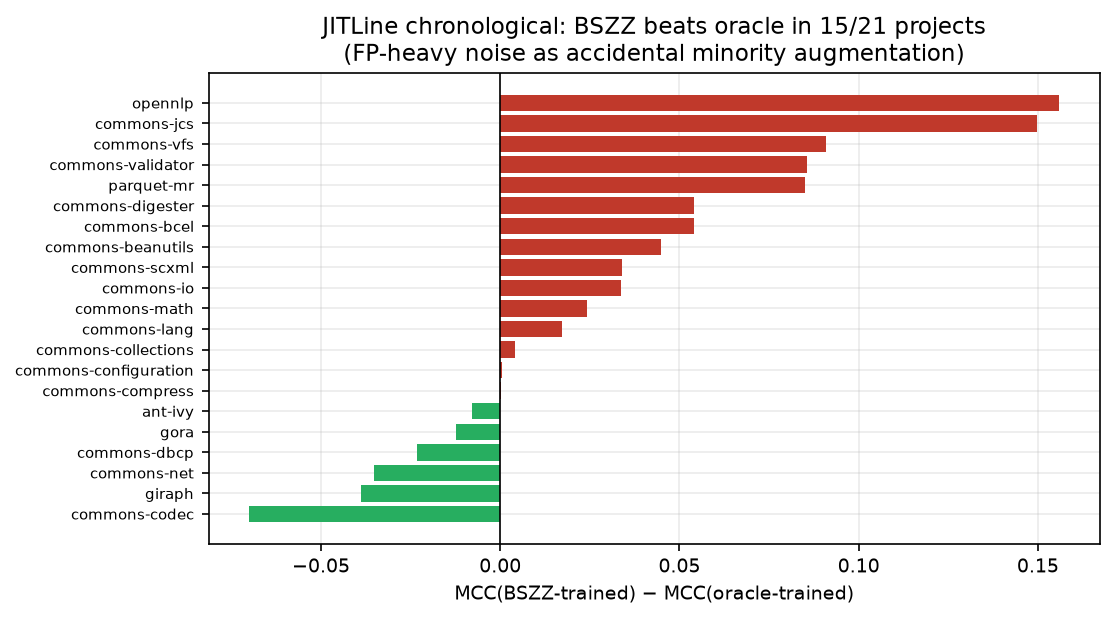
\includegraphics[width=\linewidth,keepaspectratio]{figures/f8_jitline_anomaly.png}
\label{fig:f8_jitline_anomaly}
\caption{Per-project B-SZZ-minus-reference gap for JITLine}
\end{figure}

\textbf{Figure 5.6 --- Reading the figure.} One bar per project. Bars to
the right are projects where training on \emph{noisy} B-SZZ labels beat
training on the reference labels; bars to the left are the reverse.

\textbf{The phenomenon is real, not seed noise.} 97.7\% of the
between-project variance is genuine rather than seed variation; 16 of 21
projects show a gap more than two standard errors from zero; and it
survives all four threshold-selection protocols tested.

\textbf{But no project characteristic predicts where it happens.}

\begin{figure}
\centering
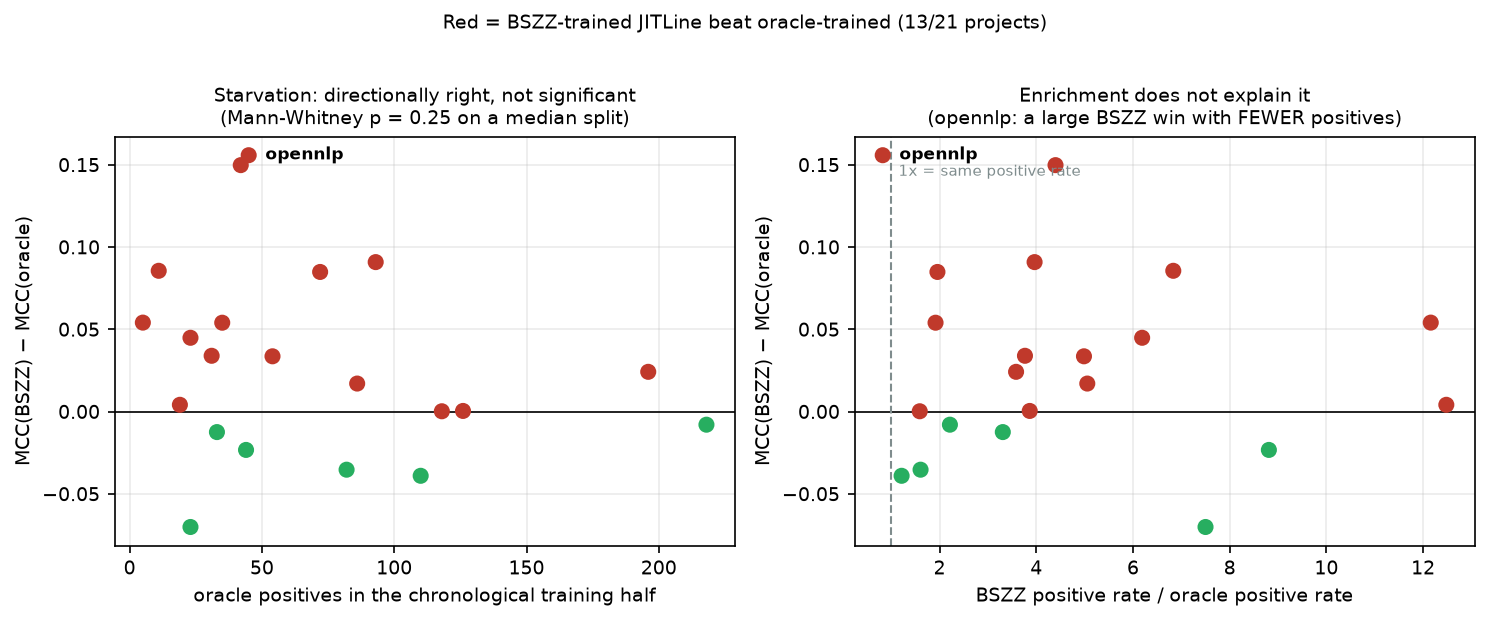
\includegraphics[width=\linewidth,keepaspectratio]{figures/f9_anomaly_predictors.png}
\label{fig:f9_anomaly_predictors}
\caption{What predicts the anomaly --- nothing does}
\end{figure}

\textbf{Figure 5.7 --- Reading the figure.} \emph{Left:} the gap against
how many defect examples a project supplies for training --- if minority
starvation were the mechanism, the points would slope clearly downward.
\emph{Right:} the gap against how many extra positive labels B-SZZ
supplies. \texttt{opennlp} is annotated on both panels because it sits
on the wrong side of the 1\ensuremath{\times} line.

\begin{longtable}[]{@{}lll@{}}
\toprule\noalign{}
Predictor & Spearman \ensuremath{\rho} with gap & \emph{p} \\
\midrule\noalign{}
\endhead
\bottomrule\noalign{}
\endlastfoot
Training-half defect examples & \ensuremath{-}0.336 & 0.14 \\
Total defect examples & \ensuremath{-}0.216 & 0.35 \\
Label-arrival coverage & \ensuremath{-}0.175 & 0.45 \\
Number of commits & \ensuremath{-}0.149 & 0.52 \\
B-SZZ precision & \ensuremath{-}0.135 & 0.56 \\
B-SZZ recall & \ensuremath{-}0.108 & 0.64 \\
Enrichment (B-SZZ rate \ensuremath{\div} reference rate) & +0.066 & 0.78 \\
Reference defect rate & \ensuremath{-}0.056 & 0.81 \\
B-SZZ flag rate & \ensuremath{-}0.029 & 0.90 \\
\end{longtable}

\textbf{Not one reaches even uncorrected significance}, across 18 tests
where roughly one would be expected to by chance.

Two mechanisms point the right way without reaching significance.
\emph{Minority enrichment}: projects with few training defects gain
+0.0479 against +0.0015 for positive-rich projects (Mann--Whitney
\emph{p} = 0.245). \emph{Headroom}: B-SZZ helps most where the
reference-trained model is already weak (reference MCC 0.093 in
B-SZZ-win projects against 0.119 elsewhere, \emph{p} = 0.137). These are
not independent --- fewer defects \emph{causes} a weaker model --- so
they are one hypothesis rather than two.

\begin{quote}
\textbf{A counter-example the enrichment story cannot absorb.}
\texttt{opennlp} is the second-largest B-SZZ win (+0.162 \ensuremath{\pm} 0.010), yet
B-SZZ flags a \emph{lower} rate there than the reference --- 6.91\%
against 8.38\%, an enrichment of 0.82\ensuremath{\times}. There is no extra minority mass
to explain the gain.
\end{quote}

\textbf{It is a batch phenomenon only.} Under streaming, the reference
beats B-SZZ in 18 of 21 projects; the anomaly does not carry over, which
suggests batch and online learners are sensitive to different properties
of the labels --- itself a question for the later phases.

\textbf{How this is stated in this report:} the phenomenon is robust and
worth reporting; the \emph{mechanism} is not established, and no
mechanism is claimed.

\section{5.4 Robustness}\label{robustness}

\textbf{Estimator and fading factor.} The label-source conclusion was
re-examined across fading factors 0.90--0.999 (effective windows
10--1000 commits) crossed with warm-up skips of 0/5/10/25\% --- 20
settings \ensuremath{\times} 6 variants = 120 comparisons. In \textbf{120 of 120}, the
Hodges--Lehmann estimate favours the reference labels, the bootstrap
interval excludes zero, and the comparison survives \emph{grid-wide}
Holm correction.

This is one result re-examined under different analytical choices, not
120 findings, and grid-wide correction is applied so the framing cannot
be mistaken.

\textbf{Project weighting.} Every figure is an unweighted mean over
projects carrying between 19 and 335 reference defects; eight of 21
carry fewer than 25 in the chronological test half. Re-running the
headline contrasts with the smallest projects excluded:

\begin{longtable}[]{@{}lll@{}}
\toprule\noalign{}
Claim & All 21 & \ensuremath{\geq} 25 defects (\emph{n} = 13) \\
\midrule\noalign{}
\endhead
\bottomrule\noalign{}
\endlastfoot
\emph{k}-fold inflation & +0.137 & \textbf{+0.136} \\
Self-scoring gap (\emph{k}-fold) & +0.230 & \textbf{+0.232} \\
Label source (reference vs B-SZZ) & +0.041 & \textbf{+0.043} \\
\end{longtable}

No estimate moves by more than 0.002 MCC and all three still survive
correction. \textbf{The conclusions are not artefacts of the small
projects.} One claim does weaken: the self-scoring gap under the
\emph{chronological} regime falls from +0.098 to +0.075 and loses
significance --- not the headline, but the deployment-relevant regime,
and reported here rather than omitted.

\section{5.5 Discussion --- answering
RQ2}\label{discussion-answering-rq2}

\textbf{The label source shifts measured performance, and the shift is
significant under every regime that permits a fair test.} Under
realistic streaming the penalty for training on SZZ rather than the
reference is 0.034--0.064 MCC, against a deployable baseline of roughly
0.097 --- between a third and two-thirds of the available signal.

\textbf{But the regime shifts it more.} Moving from \emph{k}-fold to
chronological costs JITLine 0.137. Removing circular scoring costs a
further 0.230. \textbf{The two protocol effects together are roughly
nine times the label-source effect.}

This inverts the question the chapter set out to ask. Phase 2 was
designed to measure what SZZ noise costs. What it found is that
\textbf{the cost of SZZ noise is small relative to the cost of the
field's evaluation conventions} --- and that the two interact, because
self-scoring is only possible \emph{because} the labels are heuristic.
If the field had ground truth, it would score against it, and the +0.230
gap could not exist.

\textbf{The implication for reading published results.} A JIT-SDP result
reported under random \emph{k}-fold with self-scored SZZ labels is not a
measurement of defect-prediction capability. On this corpus the
difference between that protocol and a defensible one is 0.41 versus
0.10 MCC. Any comparison between published models measured this way is
confounded by capacity-dependent inflation, since the artefact is larger
for models with more capacity to exploit it.

\textbf{What Phase 2 could not determine.} Which \emph{kind} of SZZ
error does the damage. The label-source gap shows that label quality
matters; it does not show whether the cost comes from the false
positives SZZ invents or the defects it misses. The gap's failure to
track recall (\ensuremath{-}0.18) rules out the simplest explanation and leaves the
question open.

That question is the subject of Phase 3, and answering it requires an
intervention rather than an observation. Chapter 6 sets out the design.
